\nsection{Prime Factors}

\wwwurl{en.wikipedia.org/wiki/Prime_factor}

It is well known that any positive integer has a single {\it unique}
prime factorization, e.g.:

$210 = 7 \times 5 \times 3 \times 2$ (the numbers $7,5,3$ and
$2$ are all prime).

$117 = 13 \times 3 \times 3$ (the numbers $13$ and $3$ are all
prime).

$197$ is prime, so has only itself (and $1$, which we ignore)
as a factor.

\begin{exercise}
Write a program that, for any given positive integer input
using \verb^argv[1]^, lists the prime factors, e.g.:

\begin{terminaloutput}
[campbell@icy]% ./primefacts 210
7 5 3 2

[campbell@icy]% ./primefacts 117
13 3 3
\end{terminaloutput}
\end{exercise}

\begin{exercise}
To make the output of the above program briefer,
many prefer to show the factors
expressed by their power, as in~:
\[
768 = 2 \times 2 \times 2 \times 2 \times 2 \times 2 \times 2 \times 3
\]
could be better expressed as~:
\[
768 = 2^8 \times 3
\]
Write a program to show the factorisation of a number
in this more compact style~:
\begin{terminaloutput}
 % ./primefactors 27000
27000 = 1 x 2^3 x 3^3 x 5^3
 % ./primefactors 31          
31 = 1 x 31
 % ./primefactors 38654705664
38654705664 = 1 x 2^32 x 3^2
\end{terminaloutput}
\end{exercise}


\begin{exercise}

\strut\vspace*{0.2cm}

\toohard

For a beautiful visualisation of prime factors, see:\\
\wwwurl{www.datapointed.net/visualizations/math/factorization/animated-diagrams}
Adapt the program above to output a
pattern similar to the animated display above, using SDL, but
only for a single number given via \verb^argv[1]^.
\begin{center}
\scalebox{0.3}{
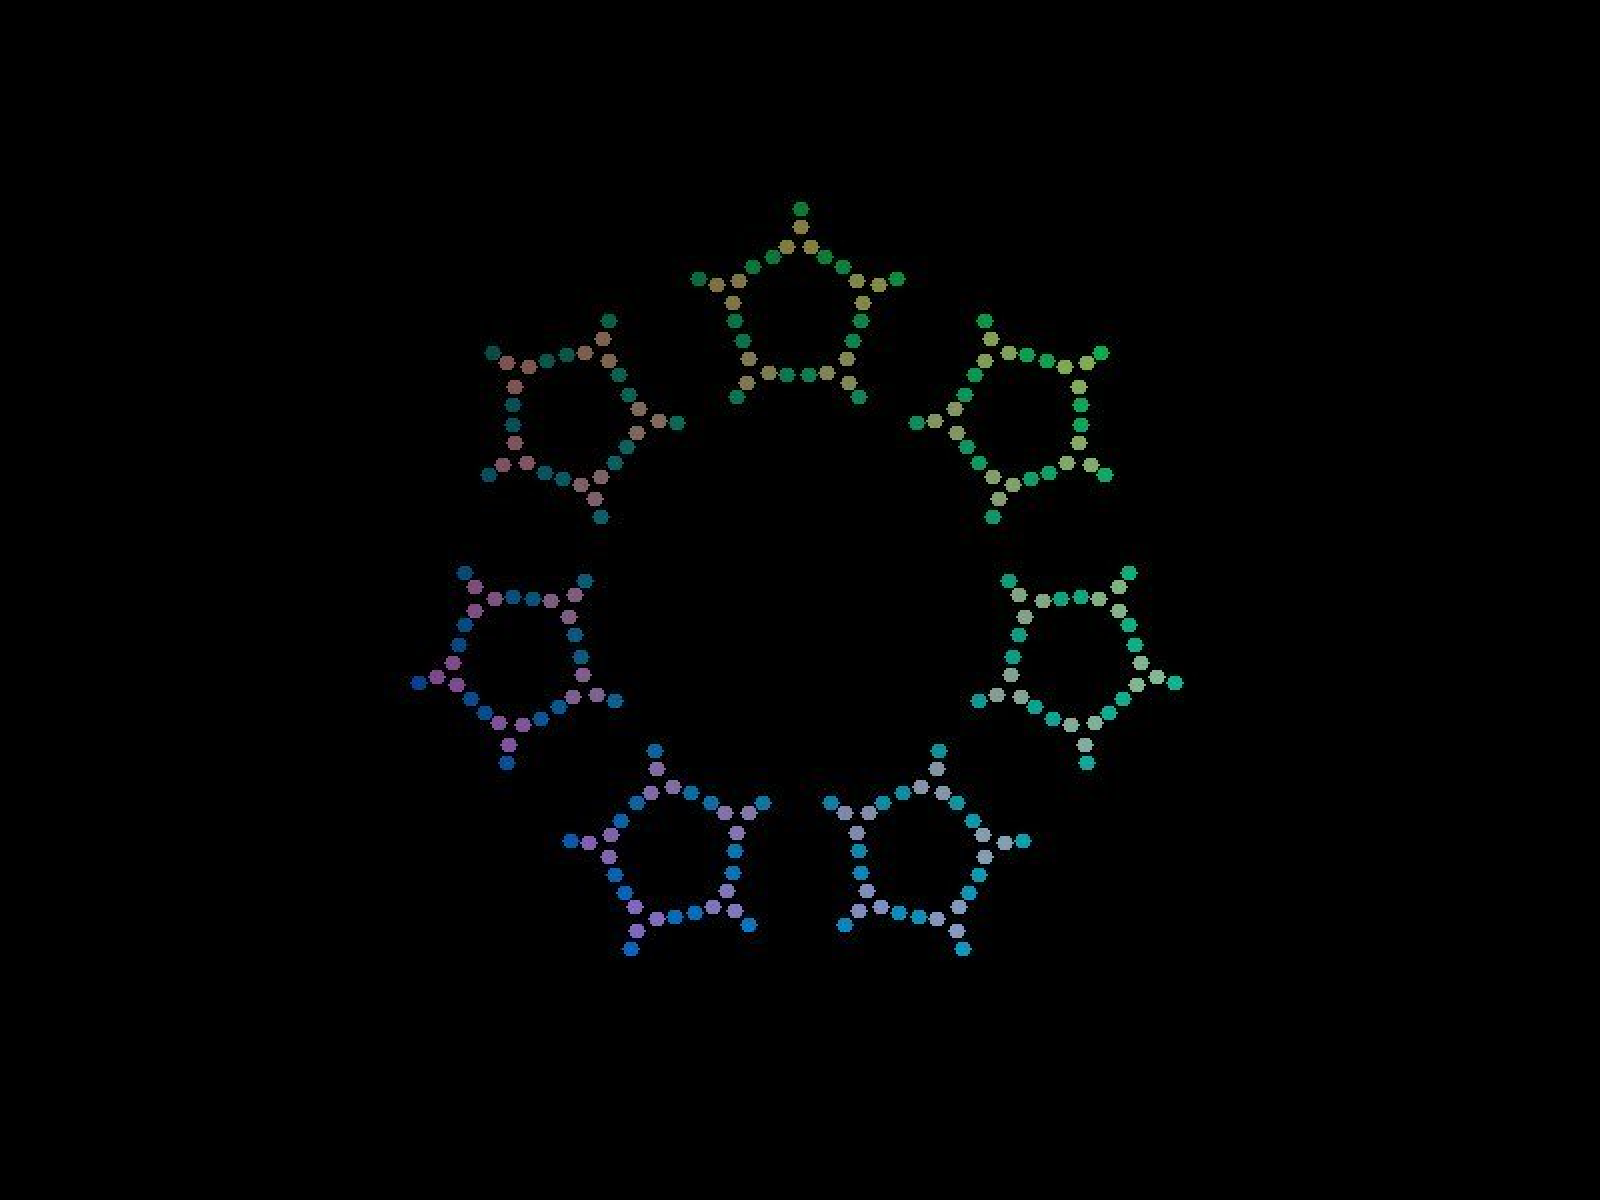
\includegraphics{./primevis.pdf}
}
\end{center}
\end{exercise}
